\chapter{The FPGA flow: from text to silicon}
\label{ch:fpga-flow}

Every chapter until now treated Verilog as something that lives inside a
simulator. An FPGA is where Verilog stops being a description and becomes
physical hardware: the text you write is compiled into a bitstream that
configures millions of tiny switches inside a real chip. This chapter walks the
whole flow --- what an FPGA actually is, what each toolchain stage does to your
code, how to write constraints so the tools know where your pins and clocks
are, and how to read the reports the tools hand back. We use the
Tang~Nano~9K, a board cheap enough to buy with pocket money, as the running
example. Every simulation and synthesis step is run for real below; the
physical board steps are marked honestly because there is no board attached to
the machine writing this.

\section{What an FPGA is}

\index{FPGA}\index{LUT}\index{BRAM}\index{IOB}
A microcontroller runs instructions one at a time. An FPGA \emph{contains}
hardware: a fabric of small programmable logic blocks surrounded by a sea of
programmable wiring. Figure~\ref{fig:fabric} shows the layout.

\begin{figure}[htbp]\centering
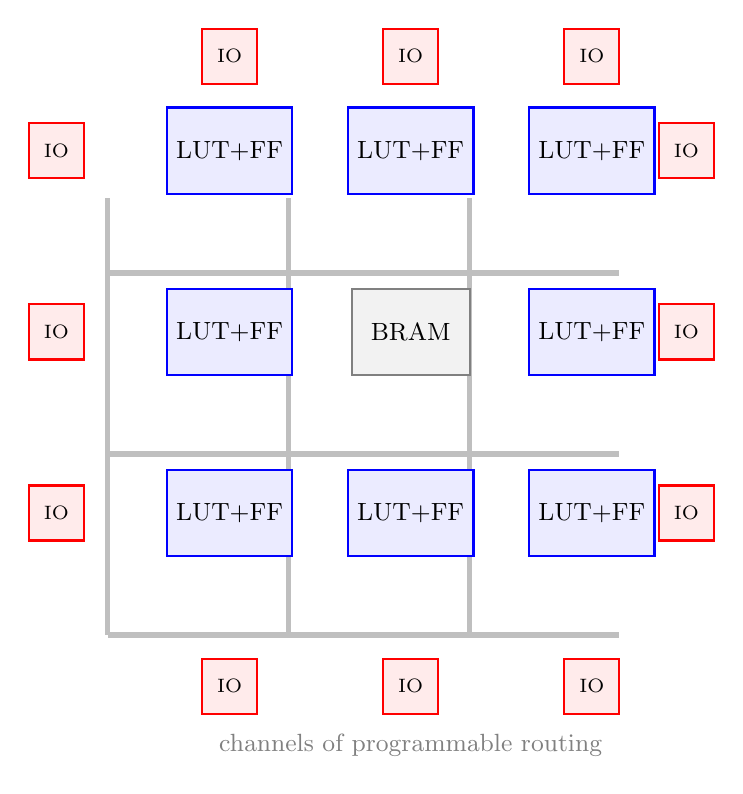
\begin{tikzpicture}[x=1cm,y=1cm,
  clb/.style={draw=blue, thick, fill=blue!8, minimum width=1.5cm, minimum height=1.1cm, font=\small},
  blk/.style={draw=gray, thick, fill=gray!10, minimum width=1.5cm, minimum height=1.1cm, font=\small},
  iob/.style={draw=red, thick, fill=red!8, minimum width=0.7cm, minimum height=0.7cm, font=\scriptsize}]
% routing channels
\foreach \x in {0,2.3,4.6} {\draw[gray!50, line width=2pt] (\x-0.95,-0.95) -- (\x-0.95,4.6);}
\foreach \y in {0,2.3,4.6} {\draw[gray!50, line width=2pt] (-0.95,\y-0.95) -- (5.55,\y-0.95);}
% CLB grid
\node[clb] at (0.6,0.6) {LUT+FF}; \node[clb] at (2.9,0.6) {LUT+FF}; \node[clb] at (5.2,0.6) {LUT+FF};
\node[clb] at (0.6,2.9) {LUT+FF}; \node[blk] at (2.9,2.9) {BRAM};  \node[clb] at (5.2,2.9) {LUT+FF};
\node[clb] at (0.6,5.2) {LUT+FF}; \node[clb] at (2.9,5.2) {LUT+FF}; \node[clb] at (5.2,5.2) {LUT+FF};
% IO ring
\foreach \p in {(0.6,-1.6),(2.9,-1.6),(5.2,-1.6),(-1.6,0.6),(-1.6,2.9),(-1.6,5.2),(0.6,6.4),(2.9,6.4),(5.2,6.4),(6.4,0.6),(6.4,2.9),(6.4,5.2)} \node[iob] at \p {IO};
\node[gray, font=\small] at (2.9,-2.35) {channels of programmable routing};
\end{tikzpicture}

\caption{The FPGA fabric. Look at the regularity: identical logic tiles in a
grid, routing channels between them, I/O blocks around the edge, and a few
bigger blocks (block RAM, and on some chips multipliers or a clock manager)
dropped into the grid. Place-and-route is literally the problem of deciding
which tile runs each piece of your design and how the channels connect them.}
\label{fig:fabric}
\end{figure}

The tile itself is built around two elements:

\begin{description}
\item[LUT --- look-up table.] The universal gate. A $k$-input LUT is just a
$2^k$-entry memory: feed it an address made of your input wires and it returns
the stored bit. To implement \emph{any} Boolean function of $k$ variables, you
program the $2^k$ SRAM cells with the truth table --- Figure~\ref{fig:lut}.
That is the entire trick: no physical gates get built, the \emph{answer table}
is stored.
\item[Flip-flops.] Each LUT output feeds a configurable flip-flop, so the tile
can be purely combinational (LUT bypasses the flop) or registered (LUT feeds
the flop). Your \texttt{always @(posedge clk)} blocks become these flops.
\end{description}

Around them: \emph{routing} (a programmable mesh --- connections are made by
opening and closing switch points, which is why timing is unpredictable until
routing is done), \emph{block RAM} (real SRAM arrays, much denser than building
memory from flops), \emph{I/O blocks} (configurable pin drivers: voltage
levels, pull-ups, sometimes serdes), and usually a \emph{clock manager} (PLL)
to multiply or divide the board's oscillator.

\begin{figure}[htbp]\centering
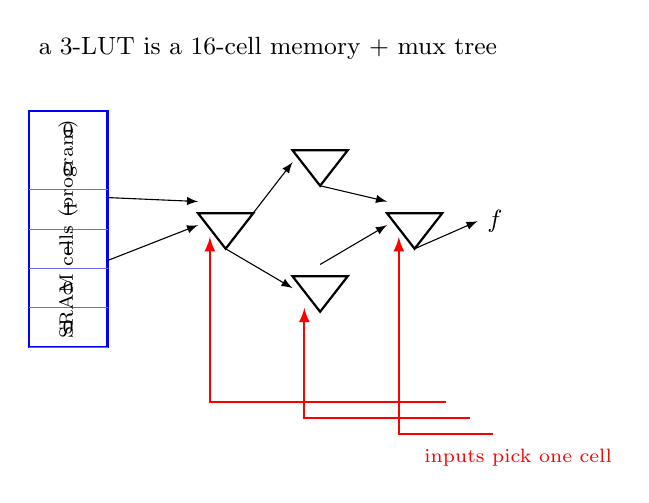
\begin{tikzpicture}[x=1cm,y=1cm, >=latex]
\node[font=\small, anchor=west] at (-0.3,3.3) {a 3-LUT is a 16-cell memory + mux tree};
% SRAM column
\draw[thick, blue] (-0.3,-0.5) rectangle (0.7,2.5);
\foreach \y in {0,0.5,...,2.49} \draw[blue!60] (-0.3,\y-0.5) -- (0.7,\y-0.5);
\node[font=\scriptsize, rotate=90] at (0.2,1.0) {SRAM cells (program)};
\foreach \y/\v in {-0.5/0,0.0/0,0.5/1,1.0/1,1.5/0,2.0/0}
  \node[font=\scriptsize] at (0.2,\y+0.25) {\v};
% mux symbols: drawn triangles (no shapes lib)
\foreach \p in {(2.2,0.75),(3.4,-0.05),(3.4,1.55),(4.6,0.75)}
  \draw[thick] \p -- ++(-0.35,0.45) -- ++(0.7,0) -- cycle;
\draw[->] (0.7,0.6) -- (1.85,1.05); \draw[->] (0.7,1.4) -- (1.85,1.35);
\draw[->] (2.2,0.75) -- (3.05,0.25); \draw[->] (2.2,0.75) -- (3.05,1.85);
\draw[->] (3.4,0.55) -- (4.25,1.05); \draw[->] (3.4,1.55) -- (4.25,1.35);
\draw[->] (4.6,0.75) -- (5.4,1.1) node[anchor=west, font=\small] {$f$};
\draw[->, red, thick] (5.0,-1.2) -| (2.0,-0.6) -- (2.0,0.9);
\draw[->, red, thick] (5.3,-1.4) -| (3.2,-0.7) -- (3.2,0.0);
\draw[->, red, thick] (5.6,-1.6) -| (4.4,-0.8) -- (4.4,0.9);
\node[red, font=\scriptsize, anchor=west] at (4.6,-1.9) {inputs pick one cell};
\end{tikzpicture}

\caption{A LUT is SRAM plus a mux tree. The input bits act as the address and
select exactly one stored configuration bit. Change the stored bits and you
change the function --- AND, XOR, majority, anything of the same arity.}
\label{fig:lut}
\end{figure}

\begin{example}[How many LUTs is your function?]
A 4-input function needs $2^4=16$ stored bits: one 4-LUT. A 6-input function
needs 64 bits --- too big for one 4-LUT, so the tools chain LUTs together with
extra mux stages (that is what the \texttt{MUX2\_LUT5/6/7/8} cells you will see
in the synthesis report are). Exercise: a 32-bit equality comparator is a
6-input function per output bit reduced AND-wise --- how wide is the tree?
\end{example}

\section{The toolchain: five stages}

\begin{figure}[htbp]\centering
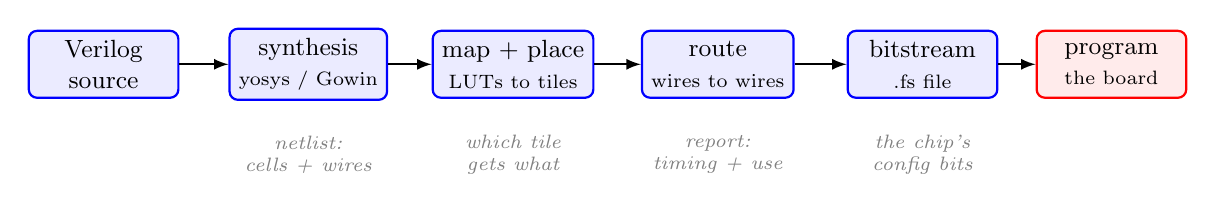
\begin{tikzpicture}[x=1cm,y=1cm, >=latex,
  stage/.style={draw=blue, thick, fill=blue!8, rounded corners=3pt, minimum width=1.9cm, minimum height=0.85cm, font=\small, align=center},
  stagenote/.style={font=\scriptsize\itshape, text=gray, align=center}]
\node[stage] (src) at (0,0) {Verilog\\ source};
\node[stage] (syn) at (2.6,0) {synthesis\\ \scriptsize yosys / Gowin};
\node[stage] (map) at (5.2,0) {map + place\\ \scriptsize LUTs to tiles};
\node[stage] (par) at (7.8,0) {route\\ \scriptsize wires to wires};
\node[stage] (bit) at (10.4,0) {bitstream\\ \scriptsize .fs file};
\node[stage, draw=red, fill=red!8] (bd) at (12.8,0) {program\\ \scriptsize the board};
\foreach \a/\b in {src/syn, syn/map, map/par, par/bit, bit/bd}
  \draw[->, thick] (\a) -- (\b);
\node[stagenote] at (2.6,-1.15) {netlist:\\ cells + wires};
\node[stagenote] at (5.2,-1.15) {which tile\\ gets what};
\node[stagenote] at (7.8,-1.15) {report:\\ timing + use};
\node[stagenote] at (10.4,-1.15) {the chip's\\ config bits};
\end{tikzpicture}

\caption{The FPGA build pipeline. Each stage eats the previous stage's output
and produces something closer to silicon: text $\to$ generic cells $\to$
specific tiles $\to$ routed wires $\to$ a bitstream the chip loads at boot.}
\label{fig:flow}
\end{figure}

\begin{description}
\item[Synthesis] reads your Verilog and produces a netlist: real cell types
(LUTs, flops, BRAMs) and the wires between them. This is where
\texttt{cnt <= cnt + 1} becomes 24 adder cells and 24 flip-flops.
\item[Map/place] assigns each cell to a physical tile on the chip.
\item[Route] connects the tiles through the programmable channels and produces
the timing report: did every register-to-register path fit inside one clock
period?
\item[Bitstream generation] packs the final configuration into a file
(\texttt{.fs} on Gowin parts) --- literally the contents of all the SRAM cells
and switch points.
\item[Program] writes the bitstream to the board, either to SRAM (lost on power
cycle) or to the onboard flash (survives).
\end{description}

Two toolchains reach the Tang~Nano~9K: Gowin's own IDE (GW\_EDA, requires a
free licence --- \url{https://www.gowinsemi.com/en/support/home/}, verified reachable 2026-10-10) and the
fully open path \texttt{yosys} + \texttt{nextpnr-himbaechel} + \texttt{apicula}
+ \texttt{openFPGALoader} \cite{apicula}. This chapter uses \texttt{yosys}
0.69's \texttt{synth\_gowin} for the synthesis stage, which is the real
synthesis pass for this chip family; place, route, and board programming are
described but not run here --- no board is attached to this machine, and the
Gowin P\&R binary is not installed. Everything marked \emph{sim} below is a
real captured run; everything marked \emph{on hardware} is the step you would
run yourself.

\section{Hello, LED: blinky}

The FPGA hello-world is a blinking LED. There is no sleep() --- you make time
by counting clocks. The board's oscillator runs at 27\,MHz, so
$2^{23}$ ticks $\approx$ 0.31\,s: wire the LED to counter bit~23 and it blinks
about twice a second.

\begin{lstlisting}[language=Verilog]
module blinky(clk, led);
  input clk; output led;
  reg [23:0] cnt = 0;
  always @(posedge clk) cnt <= cnt + 1'b1;
  assign led = cnt[23];        // the slowest counter bit IS the blink
endmodule
\end{lstlisting}

\begin{example}[Blinky, simulated first]
Never program a board you haven't simulated. The full 24-bit counter would
need millions of simulated clocks, so the testbench instantiates a scaled
twin (\texttt{led = cnt[3]}): same structure, a period you can watch.

\begin{lstlisting}
t=  0 cnt=0000 led=0
t= 25 cnt=0011 led=0
t= 65 cnt=0111 led=0
t= 75 cnt=1000 led=1
t=135 cnt=1110 led=1
t=155 cnt=0000 led=0
\end{lstlisting}

The LED is exactly the value of the chosen counter bit --- the entire design
works. This is also the honest preview of the hardware run: on the board, the
same logic at bit~23 is a $\sim$3\,s square wave.
\end{example}

\begin{figure}[htbp]\centering
\begin{tikzpicture}
\begin{axis}[width=0.85\linewidth, height=4.2cm, xlabel={$t$ (ns)},
  xmin=0, xmax=175, ymin=-0.3, ymax=1.4, clip=false,
  ytick={0,1}, yticklabels={0,1}, axis lines=left]
\addplot[const plot, thick, blue] table[x=t,y=v] {figures/ch13/ch13_blink.dat};
\node[anchor=east, font=\small] at (axis cs:0,0.5) {\sf led};
\node[font=\scriptsize, text=gray] at (axis cs:115,1.15) {bit 3 high for 8 clocks};
\end{axis}
\end{tikzpicture}

\caption{Blinky in simulation (scaled twin): \texttt{led} follows counter
bit~3, high for 8 clocks out of every 16. On hardware it is bit~23, high for
$2^{23}$ clocks out of every $2^{24}$ --- same shape, 3-million-times slower.}
\label{fig:wave}
\end{figure}

\begin{example}[Blinky through synthesis --- reading the stat report]
Strategy: run the module through \texttt{synth\_gowin} and actually read the
\texttt{stat} block instead of skimming it. Real output:

\begin{lstlisting}
=== blinky ===
       55 wires       78 wire bits        2 ports
       53 cells
       24   ALU
       24   DFF
        1   GND
        1   IBUF
        1   LUT1
        1   OBUF
        1   VCC
\end{lstlisting}

Every line is a fact about your code. \textbf{24 DFF}: one flip-flop per
counter bit, exactly as written. \textbf{24 ALU}: Gowin maps \texttt{+1} onto
the tiles' fast-carry arithmetic cells rather than LUTs. \textbf{1 LUT1}: one
1-input LUT remains to wire bit~23 out. \textbf{IBUF/OBUF}: the input clock pad
and output LED pad --- your two ports became I/O blocks. \textbf{GND/VCC}: tie
cells for constants. Nothing here is mysterious once you read it line by line.
\end{example}

\section{Counters, buses, and real area}

\begin{example}[A 6-LED counter with enable and terminal count]
Strategy: write it like ch10 taught (one clocked always block, nonblocking),
simulate the scaled twin, then synthesize and compare sizes.

\begin{lstlisting}[language=Verilog]
module counter6 #(parameter W = 27, parameter TOP = 13500000) (
  input clk, input en,
  output reg [5:0] leds = 0, output reg tc = 0);
  reg [W-1:0] div = 0;
  always @(posedge clk) begin
    tc <= 0;
    if (en) begin
      if (div == TOP) begin
        div <= 0; leds <= leds + 1'b1; tc <= 1;
      end else div <= div + 1'b1;
    end
  end
endmodule
\end{lstlisting}

Simulated (\texttt{W=4}, terminal every 16 clocks --- same logic, short wait):

\begin{lstlisting}
t= 12 en=1 div=0 leds=000000 tc=0
t=155 en=1 div=14 leds=000000 tc=0
t=165 en=1 div=0 leds=000001 tc=1
t=175 en=1 div=1 leds=000001 tc=0
t=212 en=0 div=4 leds=000001 tc=0
\end{lstlisting}

Terminal count pulses once per wrap, \texttt{leds} increments, and
\texttt{en=0} freezes everything --- all verified on tape. Now the cost:

\begin{lstlisting}
=== counter6 ===
      256 wires      335 wire bits        4 ports
      262 cells
      102   LUT1       10   LUT2        9   LUT3       32   LUT4
       57   MUX2_LUT5  25   MUX2_LUT6  12   MUX2_LUT7   5   MUX2_LUT8
        7   OBUF        2   IBUF        1   GND
       34 submodules:  6 DFFE  1 DFFR  27 DFFRE
\end{lstlisting}

Compare with blinky honestly: flops went $24\to34$ (27 divider bits + 6 LED
bits + \texttt{tc}), but LUTs went $1\to153$ plus 99 wide mux cells --- the
27-bit equality compare (\texttt{div == TOP}) is where the area went. \emph{An
equality test against a magic number is a wide AND}, and you are paying for it
in fabric. A cheaper idiom is to load the period and count down to zero
(exercise~8).
\end{example}

\begin{exercise}[easy]
In the counter6 stat report, what produced the 7 \texttt{OBUF} cells? Name
each pin they correspond to.
\end{exercise}

\section{UART: talking to the outside world}

Blinky proves the fabric works; UART proves you can \emph{communicate}. A UART
frame is one start bit (low), 8 data bits LSB-first, one stop bit (high) ---
Figure~\ref{fig:uart}. At 115200 baud on a 27\,MHz clock each bit lasts
$27\times10^6/115200 \approx 234$ clocks.

\begin{figure}[htbp]\centering
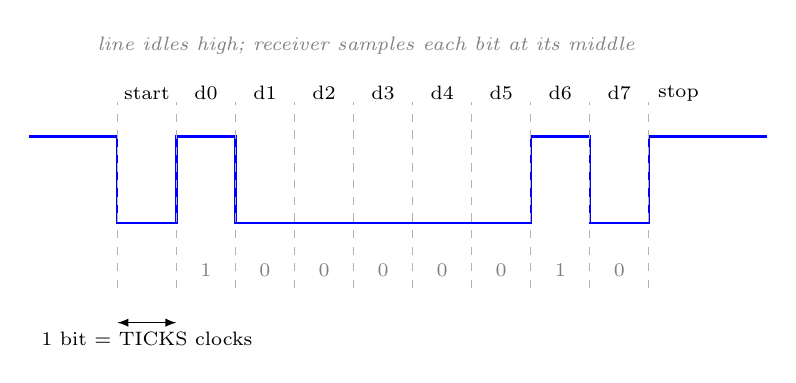
\begin{tikzpicture}[x=0.75cm,y=1.1cm, >=latex]
% frame for 'A' = 0x41, LSB first: idle 1 | start 0 | 1,0,0,0,0,0,1,0 | stop 1
\draw[thick, blue] (-0.5,1) -- (1,1) -- (1,0) -- (2,0) -- (2,1) -- (3,1)
  -- (3,0) -- (8,0) -- (8,1) -- (9,1) -- (9,0) -- (10,0) -- (10,1) -- (12,1);
\foreach \x/\n in {1.5/start,2.5/{d0},3.5/{d1},4.5/{d2},5.5/{d3},6.5/{d4},7.5/{d5},8.5/{d6},9.5/{d7},10.5/stop}
  \node[font=\scriptsize] at (\x,1.5) {\n};
\foreach \x/\v in {2.5/1,3.5/0,4.5/0,5.5/0,6.5/0,7.5/0,8.5/1,9.5/0}
  \node[font=\scriptsize, text=gray] at (\x,-0.55) {\v};
\foreach \x in {1,...,10} \draw[gray!60, dashed] (\x,-0.75) -- (\x,1.4);
\draw[<->] (1,-1.15) -- (2,-1.15) node[midway, below, font=\scriptsize] {1 bit = TICKS clocks};
\node[font=\scriptsize\itshape, anchor=west, gray] at (0.5,2.05)
  {line idles high; receiver samples each bit at its middle};
\end{tikzpicture}

\caption{One UART frame sending \texttt{'A'} (\texttt{0x41}). Notice: the line
rests high, the start bit pulls it low, data goes out least-significant-bit
first, and a full bit-time of stop ends the frame. The receiver's job is to
find the start edge and sample each bit at its middle.}
\label{fig:uart}
\end{figure}

\begin{example}[A minimal UART transmitter, verified by decoding]
Strategy: build the smallest honest transmitter (a shift register + a baud
counter), then verify it the hard way --- the testbench samples the wire at
mid-bit and reconstructs the byte, rather than trusting \texttt{\$monitor}.

\begin{lstlisting}[language=Verilog]
module uart_tx #(parameter TICKS = 234) (clk, start, data, tx, busy);
  input clk, start; input [7:0] data;
  output reg tx; output reg busy;
  reg [8:0] cnt;  reg [3:0] bitn;  reg [7:0] shreg;
  initial begin tx = 1; busy = 0; cnt = 0; bitn = 0; shreg = 0; end
  always @(posedge clk)
    if (!busy) begin
      tx <= 1;
      if (start) begin busy <= 1; shreg <= data;
                      cnt <= 0; bitn <= 0; tx <= 0; end
    end else if (cnt == TICKS - 1) begin
      cnt <= 0;
      if (bitn == 8) begin busy <= 0; tx <= 1; end
      else begin tx <= shreg[0]; shreg <= {1'b0, shreg[7:1]};
                 bitn <= bitn + 1; end
    end else cnt <= cnt + 1;
endmodule
\end{lstlisting}

The testbench (\texttt{TICKS=8} for speed) arms the decoder \emph{before}
applying the stimulus --- remember the missed-edge bug from ch12 --- then
samples mid-bit eight times:

\begin{lstlisting}
t=  3 busy=1 bit=0 tx=0
t= 19 busy=1 bit=1 tx=1
t= 35 busy=1 bit=2 tx=0
t=115 busy=1 bit=7 tx=1
t=131 busy=1 bit=8 tx=0
t=147 busy=0 bit=8 tx=1
decoded byte = 41 (want 41), busy=0
PASS: UART frame decoded
\end{lstlisting}

The wire really carried \texttt{0x41}: low for one start period, high for
\texttt{d0}, low through \texttt{d1..d5}, high for \texttt{d6}, low for
\texttt{d7}, high for stop. A transmitter that only \emph{looks} right is
suspect; one the bench decoded bit-by-bit is evidence.
\end{example}

\begin{exercise}[medium]
At 115200 baud and TICKS=234, what is the actual baud rate and the per-frame
error? At 10 bits per frame, how many frames until a receiver sampling at true
mid-bit drifts by half a bit?
\end{exercise}

\section{Constraints: telling the tools the truth}

The tools cannot guess where your ports physically live or how fast your clock
runs. Two files carry that truth.

\begin{lstlisting}[caption={Physical constraints (\texttt{ch13\_tangnano.cst}) ---
pin numbers from the Sipeed Tang~Nano~9K schematic \cite{tangnano9k}; check
your board revision before trusting them.}]
IO_LOC "clk"  52;          // the 27 MHz oscillator pin
IO_LOC "led"  10;          // onboard LED1
IO_LOC "leds[0]" 11;       // .. LED6 are 11,13,14,15,16
IO_LOC "tx"   18;          // serial header TX
\end{lstlisting}

\begin{lstlisting}[caption={Timing constraints (\texttt{ch13\_timing.sdc}) ---
one clock line, and everything else derives from it.}]
create_clock -name clk -period 37.037 [get_ports clk]
set_input_delay  -clock clk 9.0 [all_inputs]
set_output_delay -clock clk 9.0 [all_outputs]
\end{lstlisting}

\begin{example}[Why 37.037?]
The board oscillator is 27\,MHz, so one period is $1/27\times10^6 \approx
37.037$\,ns. \texttt{create\_clock} is the single most important line in the
whole file: without it, the timing report has nothing to check against and
\emph{will happily report your design as unconstrained}. The input/output
delay lines say how much of the period external devices may steal. If the
router reports \emph{worst negative slack} (WNS) $\geq 0$, every
register-to-register path fits inside 37\,ns and the design runs at 27\,MHz;
negative slack means the slowest path needs longer --- the fix is to pipeline,
not to hope.
\end{example}

\begin{figure}[htbp]\centering
\begin{tikzpicture}[x=1cm,y=1cm, >=latex]
% clock square wave, period 2 units
\draw[thick, blue] (0,2.2) -- (0,2.9) -- (1,2.9) -- (1,2.2) -- (2,2.2) -- (2,2.9) -- (3,2.9) -- (3,2.2) -- (4,2.2) -- (4,2.9) -- (5,2.9) -- (5,2.2) -- (6,2.2) -- (6,2.9) -- (7,2.9) -- (7,2.2) -- (8,2.2);
\node[anchor=east, font=\small] at (-0.15,2.55) {\sf clk};
\draw[<->] (2,3.25) -- (4,3.25) node[midway, above, font=\small] {period $T=1/f$};
% data-valid window around the edge at x=3
\draw[fill=red!15, draw=red, thick] (2.3,0.4) rectangle (3.0,1.0);
\node[font=\scriptsize, text=red] at (2.65,1.2) {setup};
\draw[fill=amber!25, draw=amber!80!black, thick] (3.0,0.4) rectangle (3.55,1.0);
\node[font=\scriptsize, text=amber!80!black] at (3.55,1.2) {hold};
\draw[thick, gray] (3,0.2) -- (3,1.4);
\node[font=\scriptsize, gray] at (3,0.0) {edge};
\draw[->] (0,-0.5) -- (8.6,-0.5) node[anchor=west, font=\small] {$t$};
\node[font=\scriptsize\itshape, text=gray, anchor=west] at (4.4,0.7) {data must be still in the shaded window};
\node[font=\scriptsize\itshape, text=gray, anchor=west] at (4.4,0.25) {between two flops, one $T$ is the whole budget};
\end{tikzpicture}

\caption{The entire timing budget is one clock period. Between two flops,
logic must settle before the setup window opens and stay stable through the
hold window. \texttt{create\_clock} tells the tools the value of $T$; the
timing report is their verdict on whether your logic fits inside it.}
\label{fig:timing}
\end{figure}

\section{On real hardware --- and what we could not do here}
\label{sec:hardware}

On a desk with the board, the flow per project is: write
\texttt{top.v} + \texttt{.cst} + \texttt{.sdc}, run synthesis, place, route,
inspect the utilization and timing reports, generate the \texttt{.fs}
bitstream, then program with Gowin's programmer or
\texttt{openFPGALoader -b tangnano9k top.fs}. The three builds you now own map
directly: \texttt{blinky} $\to$ one LED at $\sim$3\,s; \texttt{counter6} $\to$
six LEDs counting in binary once a second; \texttt{uart\_tx} wired to a
free-running ROM of text $\to$ the serial header speaks at 115200 baud (and a
loopback wire from \texttt{tx} to an \texttt{rx} module makes the classic
echo).

\textbf{Honest marking.} The simulations and the two synthesis runs in this
chapter were executed and captured on this machine. The place-and-route, the
timing report, the bitstream, and any behaviour of a physical board were
\textbf{not} run here --- no board is attached and the Gowin place-and-route
tools are not installed. Where the text says ``on hardware,'' it is describing
the step you would perform, not a result we observed. That distinction is a
feature of the chapter, not a gap: claiming a board blinked when it never ran
is how bad lab reports start.

\begin{exercise}[hard]
For \texttt{counter6}, write the complete on-hardware checklist for
programming the Tang~Nano~9K: the four commands you run, the file each
produces, and the two numbers in the reports you must check before
touching the board.
\end{exercise}

\section{Common mistakes}

\begin{itemize}
\item \textbf{Programming before simulating.} The board gives you almost no
visibility; the testbench gives you total visibility. Program only what the
sim already proved.
\item \textbf{Believing an unconstrained design is ``timing-clean.''} No
\texttt{create\_clock} means the report has nothing to check. Silence is not
approval.
\item \textbf{Trusting pin numbers from any tutorial (including this one)
without checking the schematic.} Pin maps change between board revisions.
\item \textbf{Treating synthesis warnings as noise.} ``Inferred latch,'' ``no
driver,'' ``unused signal trimmed'' are the tools telling you your design
isn't what you think it is.
\item \textbf{Confusing sim-speed with hardware-speed.} A counter that
verifies at \texttt{W=4} must be re-read at \texttt{W=27}: the logic is
identical but the numbers, and the wait, are not.
\item \textbf{Reporting hardware results you never observed.} Mark what ran
and what didn't; ``should work'' is not ``did work.''
\end{itemize}

\section*{Exercises}

\emph{Hints and full solutions are at the end of the chapter.}

\begin{enumerate}
\item[{[}easy{]}] List the four resources inside an FPGA tile region and one
sentence on what each does.
\item[{[}easy{]}] In the blinky stat report, which cells implement the
\texttt{assign led = cnt[23]} line itself? Why is there no LUT per LED?
\item[{[}easy{]}] Name the five pipeline stages and the file type each one
produces.
\item[{[}easy{]}] The board runs at 27\,MHz. Write the
\texttt{create\_clock} line. What changes if the oscillator were 50\,MHz?
\item[{[}medium{]}] A 4-bit counter at 27\,MHz: which bit blinks at
$\sim$1.7\,Hz, which at $\sim$0.84\,Hz? Show the division.
\item[{[}medium{]}] Re-derive TICKS for 9600 baud on 27\,MHz. If you instead
round to 2813 clocks, what baud error do you introduce per frame?
\item[{[}medium{]}] Sketch the UART frame for \texttt{0xC3} on paper: mark
start, data LSB-first, stop. Then have your neighbour decode it back ---
did they get \texttt{0xC3} or a framing error?
\item[{[}medium{]}] counter6 costs 153 LUTs mostly in the
\texttt{div == TOP} compare. Rewrite it as a load-and-count-down-to-zero
divider and explain why the compare shrinks.
\item[{[}medium{]}] The timing report says WNS $= -1.4$\,ns on the path
\texttt{div[0]$\to$leds[5]}. Is the design safe at 27\,MHz? Name the one
structural change that fixes it without lowering the clock.
\item[{[}medium{]}] Explain to a beginner why \texttt{IO\_LOC "tx" 18} is not
a Verilog statement and where it is consumed instead.
\item[{[}hard{]}] Design a UART \emph{receiver}: oversample at
$16\times$ baud, find the start edge, sample each data bit once at its
middle. State exactly which of your samples double-checks the stop bit and
what a missing stop bit means.
\item[{[}hard{]}] blinky used an ALU per bit for \texttt{+1}. Prove from the
stat report that a 24-bit \emph{shift register} needs no ALUs. Write the
module and predict its cell counts before you run it.
\item[{[}hard{]}] You program the board and see \emph{nothing}: no blink, no
errors, correct bitstream. List four distinct failure causes and the one
cheapest test that distinguishes each.
\item[{[}hard{]}] Your design needs a 1024$\times$8 memory. Estimate the cost
in flops versus one BRAM block, and explain why building it from registers is
the wrong answer twice over (area \emph{and} timing).
\item[{[}hard{]}] The open toolchain (yosys/nextpnr/apicula/openFPGALoader)
replaced a vendor IDE for a whole chip family. What does each of the four
pieces contribute, and which piece had to be reverse-engineered?
\end{enumerate}

\section*{Hints and answers}

\begin{description}
\item[OBUF count (inline, easy):] 7 outputs = 6 \texttt{leds[5:0]} + 1
\texttt{tc}. Each output port becomes one output buffer.
\item[Baud error (inline, medium):] actual baud $= 27\times10^6/234 \approx
115385$, i.e.\ $+0.16$\,\%. Over a 10-bit frame the sample point drifts
$\approx 1.6$\,\% of one bit --- far inside the 50\,\% margin. Safe.
\item[Hardware checklist (inline, hard):] synth $\to$ netlist; map/place+route
$\to$ routed design + reports (check \emph{WNS $\geq 0$} and the pin report
against the schematic); bitstream $\to$ \texttt{.fs}; program. The two numbers:
WNS and LUT utilization.
\item[1.] LUT+FF tile (logic), routing channels (wires), IOB (pins), BRAM
(memory).
\item[2.] One \texttt{LUT1} (the wire to the pad) + \texttt{OBUF}; an output
needs no logic of its own.
\item[4.] \texttt{-period 37.037}; a 50\,MHz clock is \texttt{-period 20.0} ---
the whole budget shrinks and previously-passing paths may fail.
\item[5.] $27\times10^6/2^{24} \approx 1.61$\,Hz ($\approx$1.7: bit~23) and
$27\times10^6/2^{25} \approx 0.80$\,Hz ($\approx$0.84: bit~24). Carry the
powers of two, don't guess.
\item[6.] $27\times10^6/9600 = 2812.5$; TICKS=2813 gives baud 9598.9 ($-0.01$\,\%).
\item[8.] A down-counter to zero compares against a constant whose test is
``all-zero NOR'' --- still wide, but many synth tools fold it into the counter
feedback cheaper than a magic-number compare; verify by re-running the stat.
\item[9.] No --- negative slack fails at speed. Pipeline: register the
\texttt{leds} output stage so the compare path ends one flop earlier.
\item[11.] Sample mid-bit using TICKS/2 offset after the start edge; the 10th
sample checks stop $=1$, a 0 there is a \emph{framing error} (misaligned
clock).
\item[12.] Predict: 24 DFF, 0 ALU, 0--1 LUTs. \texttt{shreg <= \{shreg[22:0], shreg[23]\}} --- pure wiring into flops.
\item[13.] Clock pin wrong (test: probe clk pad); constraint file not applied
(test: reread project summary); LED polarity inverted (test: tie led to VCC);
synthesized wrong top module (test: check \texttt{-top} name).
\item[14.] $1024\times8$ flops $\approx 8192$ DFFs and a terrible mux tree;
one BRAM block does it with dedicated hardware and fast address decoding.
\end{description}

\section*{Further reading}

\begin{itemize}
\item \emph{Project Apicula} (YosysHQ), \url{github.com/YosysHQ/apicula} --- the
open bitstream-documentation effort that makes Gowin chips usable without the
vendor IDE; read the README to see what ``documented bitstream'' really means.
Intermediate. Verified 200, 2026-10-10.
\item Lushay Labs, \emph{Tang Nano series tutorials},\newline
\url{learn.lushaylabs.com/tang-nano-series} --- practical getting-started
material for this exact board, IDE setup through external RAM. Beginner.
Verified 200, 2026-10-10.
\item Sipeed, \emph{Tang Nano wiki}, \url{wiki.sipeed.com/hardware/en/tang} ---
the board family's official docs (schematics, pin maps, toolchain links).
Reference. Verified 200, 2026-10-10.
\item fpga4fun, \emph{Serial interface (RS-232)},\newline
\url{fpga4fun.com/SerialInterface.html} (site's TLS certificate has a
name mismatch; the page itself loads) ---
UART TX/RX explained at the bit level with working Verilog, matching this
chapter's section. Beginner--intermediate. Verified 200, 2026-10-10.
\item YosysHQ, \emph{Yosys manual and command reference}, \url{yosyshq.net/yosys} ---
the tool that ran every synthesis line in this chapter; the \texttt{stat} and
\texttt{synth\_gowin} docs decode the reports. Reference. Verified 200,
2026-10-10.
\item Sipeed, \emph{TangNano-9K-example} repo, \url{github.com/sipeed/TangNano-9K-example} ---
the vendor's own example set (blinky, UART, displays) for when you have the
board. Beginner. Verified 200, 2026-10-10.
\end{itemize}

\begin{rulebox}{Watch instead}
\begin{itemize}
\item ``Get Started With FPGAs and Verilog in 13 Minutes!'' --- Doctor Volt
(13:30). The same board family and the real vendor-IDE flow end to end.
Matches \S\S\ref{sec:hardware}; opened and confirmed 2026-10-10.
\url{https://youtu.be/aWm9pJ2KobA}
\item ``What's an FPGA?'' --- Charles Clayton (1:25). A one-minute
definition of LUTs, routing, and fabric --- a vocabulary warm-up, not a
walkthrough. Matches \S1; opened and confirmed 2026-10-10.
\url{https://youtu.be/iHg0mmIg0UU}
\end{itemize}
\end{rulebox}

\chapternotes{\cite{tangnano9k} is the source for the board's 27\,MHz
oscillator and pin map; \cite{apicula} for the open-toolchain stage names;
\cite{fpga4fun} for the UART bit-level conventions used here; \cite{lushay}
for the board-specific flow steps.}
